% !TEX TS-program = XeLaTeX+MakeIndex+BibTeX
% !TEX encoding = UTF-8 Unicode

\PassOptionsToPackage{unicode}{hyperref}
\PassOptionsToPackage{naturalnames}{hyperref}

\documentclass[tg]{mdtufsm}
\usepackage[brazilian]{babel}

\usepackage[T1]{fontenc}
\usepackage[utf8]{inputenc}

\usepackage{fix-cm}
\usepackage{times}
\usepackage{graphicx}
\usepackage{array}
\usepackage{listings}
\usepackage{hhline}
\usepackage{amsmath,latexsym,amssymb}
\usepackage{siunitx}
\usepackage{pdfpages}
\usepackage[inner=30mm,outer=20mm,top=30mm,bottom=20mm]{geometry}
\usepackage{subcaption}

\lstdefinelanguage{Java}{
  keywords={public, private, new, true, boolean, false, catch, void, return, null, for, switch, var, if, in, while, else, case, break, class,
  	Funcionalidade, Contexto, Dado, Quando, E, Entao, Cenario, Delineacao, Exemplos},
  keywordstyle=\color[rgb]{0.2,0.4,0.55}\bfseries,
  ndkeywords={export, throw, implements, import, this,
    @Before, @Test, @After, @Dado, @Quando, @E, @Entao, @Documented, @Retention, @Target, @Teste, @aceitacao, @rejeicao, codigoDis, nomeNovaDisciplina, relevancia, siglaInst, msgErro},
  %ndkeywords={Add, Num},
  ndkeywordstyle=\color[RGB]{218,202,66}\bfseries,
  %identifierstyle=\color{black},
  sensitive=true,
  comment=[l]{//},
  morecomment=[s]{/*}{*/},
  commentstyle=\color{purple}\ttfamily,
 % stringstyle=\color[rgb]{0.0,0.4,0.65}\ttfamily,
  stringstyle=\color[RGB]{34,128,24}\ttfamily,
  %morestring=[b]',
  morestring=[b]"
}

\lstset{
	language=Java,
	basicstyle=\tiny,
	commentstyle=\color[rgb]{0,0.2,0}\normalfont,
	frame=single,
	%texcl=true,
	numbers=left,
	showstringspaces=false,
}

\lstset{
	basicstyle=\scriptsize\ttfamily,
	tabsize=2,
	frame=single,
	breaklines=true,
	breakatwhitespace=true,
	xleftmargin=0cm,
	xrightmargin=0cm,
	literate=
		{á}{{\'a}}1 {é}{{\'e}}1 {í}{{\'i}}1 {ó}{{\'o}}1 {ú}{{\'u}}1
		{Á}{{\'A}}1 {É}{{\'E}}1 {Í}{{\'I}}1 {Ó}{{\'O}}1 {Ú}{{\'U}}1
		{à}{{\`a}}1 {è}{{\`e}}1 {ì}{{\`i}}1 {ò}{{\`o}}1 {ù}{{\`u}}1
		{À}{{\`A}}1 {È}{{\'E}}1 {Ì}{{\`I}}1 {Ò}{{\`O}}1 {Ù}{{\`U}}1
		{ä}{{\"a}}1 {ë}{{\"e}}1 {ï}{{\"i}}1 {ö}{{\"o}}1 {ü}{{\"u}}1
		{Ä}{{\"A}}1 {Ë}{{\"E}}1 {Ï}{{\"I}}1 {Ö}{{\"O}}1 {Ü}{{\"U}}1
		{â}{{\^a}}1 {ê}{{\^e}}1 {î}{{\^i}}1 {ô}{{\^o}}1 {û}{{\^u}}1
		{Â}{{\^A}}1 {Ê}{{\^E}}1 {Î}{{\^I}}1 {Ô}{{\^O}}1 {Û}{{\^U}}1
		{ã}{{\~a}}1 {Ã}{{\~A}}1 {õ}{{\~o}}1 {Õ}{{\~O}}1
		{ç}{{\c c}}1 {Ç}{{\c C}}1,
	texcl=true,
	%numbers=left,
	showstringspaces=false,
	commentstyle=\normalfont
}

\captionsetup{compatibility=false}
\geometry{a4paper}
\usepackage[hidelinks,
            bookmarksopen=true,linktoc=none,colorlinks=true,
            linkcolor=black,citecolor=black,filecolor=magenta,urlcolor=blue,
            pdftitle={Automação de Interfaces Gráficas para Modelos de Simulação de Culturas Agrícolas com Base em Linguagem de Programação Visual},
            pdfauthor={Romulo Pulcinelli Benedetti},
            pdfsubject={Trabalho de Graduação},
            pdfkeywords={Automação de Software, Linguagens de Programação Visual, Modelos de Simulação de Culturas Agrícolas, Automação de Interfaces Gráficas, Blockly}
            ]{hyperref}


%%% END Article customizations

\title{Automação de Interfaces Gráficas para Modelos de Simulação de Culturas Agrícolas com Base em Linguagem de Programação Visual}
\author{Benedetti}{Romulo Pulcinelli}
\course{Curso de Ciência da Computação}
\altcourse{Curso de Ciência da Computação}
\institute{Centro de Tecnologia}
\degree{Bacharel em Ciência da Computação}

\trabalhoNumero{}
\advisor[Profª.]{Drª.}{Charão}{Andrea Schwertner}
\orientadoratrue

\committee[Prof. Dr.]{Streck}{Nereu Augusto}{UFSM}
\committee[Prof. Dr.]{Lima}{João Vicente Ferreira}{UFSM}

\date{25}{Maio}{2016}

\keyword{Automação de Software}
\keyword{Linguagens de Programação Visual}
\keyword{Modelos de Simulação de Culturas Agrícolas}
\keyword{Automação de Interfaces Gráficas}
\keyword{Blockly}

% For Computer Modern:
%\def\Cpp{{C\nolinebreak[4]\hspace{-.05em}\raisebox{.4ex}{\tiny\bf ++}}}
% For Linux Libertine G
\def\Cpp{{C\nolinebreak[4]\raisebox{.20ex}{\small\bf++}}}

%\newcommand{\todo}[1]{\textsf{\color{red}#1}}
\newcommand{\todo}[1]{}
\graphicspath{{./images/}}

%%=============================================================================
%% Trampa para corrigir o bug do hyperref que redefine o caption das figuras e das
%% tabelas, não colocando o nome ``Figura'' antes do número do mesmo na lista
%%=============================================================================

\makeatletter

\long\def\@caption#1[#2]#3{%
  \expandafter\ifx\csname if@capstart\expandafter\endcsname
                  \csname iftrue\endcsname
    \global\let\@currentHref\hc@currentHref
  \else
    \hyper@makecurrent{\@captype}%
  \fi
  \@ifundefined{NR@gettitle}{%
    \def\@currentlabelname{#2}%
  }{%
    \NR@gettitle{#2}%
  }%
  \par\addcontentsline{\csname ext@#1\endcsname}{#1}{%
    \protect\numberline{\csname fnum@#1\endcsname ~-- }{\ignorespaces #2}%
  }%
  \begingroup
    \@parboxrestore
    \if@minipage
      \@setminipage
    \fi
    \normalsize
    \expandafter\ifx\csname if@capstart\expandafter\endcsname
                    \csname iftrue\endcsname
      \global\@capstartfalse
      \@makecaption{\csname fnum@#1\endcsname}{\ignorespaces#3}%
    \else
      \@makecaption{\csname fnum@#1\endcsname}{%
        \ignorespaces
        \ifHy@nesting
          \expandafter\hyper@@anchor\expandafter{\@currentHref}{#3}%
        \else
          \Hy@raisedlink{%
            \expandafter\hyper@@anchor\expandafter{%
              \@currentHref
            }{\relax}%
          }%
          #3%
        \fi
      }%
    \fi
    \par
  \endgroup
}

\makeatother

%\date{} % Activate to display a given date or no date (if empty), otherwise the current date is printed

\begin{document}
\maketitle
\makeapprove

\begin{abstract}
	A automação de tarefas é uma forma bastante eficiente pela qual podemos reduzir custos e aumentar a produtividade e qualidade da atividade humana. A computação por si é uma ferramenta para atingir a automação de tarefas, com vários exemplos de softwares focados em automatizar tarefas específicas sob comando do usuário, sendo a automatização destes softwares um campo a parte. Observamos a aproximação destes softwares a abordagens mais naturais ao raciocínio humano, por meio de interfaces gráficas e contextualização dos elementos com base no mundo real, tornando estes softwares menos distantes do paradigma de interação do humano com a realidade. Desta forma este trabalho objetiva abordar a utilização de tecnologias voltadas a programação visual para melhorar a abordagem de automação de tarefas, com foco em softwares gráficos de modelagem matemática agrícola, assim inserindo a atividade de automatizar estes softwares gráficos, dentro do mesmo domínio de abstração que as atividades destes softwares ocorrem.
\end{abstract}

\tableofcontents

\setlength{\baselineskip}{1.5\baselineskip}

\chapter{Introdução}

	No desenvolvimento de software, áreas de conhecimento como engenharia de software e qualidade de software
investigam processos e normas, com o objetivo de reduzir a quantia de recursos necessários e garantir a qualidade de
software produzido. Um dos produtos destas áreas, envolvendo automação, foi o campo de conhecimento de testes de software.

Sendo que o software pode realizar diversas tarefas, e estas podem assumir diversos estados, qualquer abordagem
de teste de software, numa situação ideal deveria avaliar todas estas tarefas e seus estados para fornecer as melhores
informações possíveis sobre a qualidade do software, o que facilmente pode se tornar uma tarefa repetitiva e de longa
duração e na maioria dos casos nem sempre é possível, segundo \cite[pag. 10]{myers2011art}.

% REVISAO (Andrea): usar itálico em palavras estrangeiras
Embora nem sempre seja possível testar todos os estados possíveis, é possível realizar os testes em uma faixa
conhecida e finita de estados. Nestes casos, usar ferramentas como \emph{frameworks} voltados a automatização destes testes
agiliza a tarefa de repetir os testes, como na abordagem de testes de regressão onde todos os testes devem ser
executados novamente a cada ciclo de desenvolvimento.

% REVISAO (Andrea): removi a frase abaixo pois "não o bastante" não faz sentido. Seria "não obstante"? (mesmo assim, não faria sentido)
%Não o bastante oferece uma série de vantagens tais como precisão ao reduzir a necessidade da atenção humana durante o andamento da tarefa, agilizando atividades e melhorando o aproveitamento do tempo de trabalho humano.

Alguns destes \emph{frameworks}, embora voltados a realização de testes, poderiam ser usados para automatizar programas gráficos. Um exemplo disso é o Robot Framework~\cite{robotFW}. Entretanto, são ferramentas que, apesar de cobrirem de forma bastante detalhada a automação de testes, não são as mais adequadas à modelagem da automatização de softwares gráficos, dependem de um domínio de assuntos de diversos campos da área de Ciências da computação e em muitos casos, domínio da especificação e arquitetura do software a ser automatizado ou ainda alterações a nível de codificação no programa a ser automatizado.

Já outros casos particulares de automatização focada em tarefas de TI são os próprios terminais ou ainda utilitários como \emph{shell},  \emph{make} e afins. Tratam-se de ferramentas e linguagens voltadas para automatização do desenvolvimento e de tarefas administrativas, também inadequadas à automatização de programas gráficos, seja por serem bastante limitadas a um mundo formalmente textual, pela complexidade de sua sintaxe ou ainda pela abstração focada em tarefas comuns apenas para profissionais de TI e para software que oferece interface com estes utilitários.

Existem também ferramentas destinadas à automação de software gráfico, como a linguagem \emph{script} de automatização Autoit~\cite{autoit}. Ainda assim, é uma ferramenta que exige o domínio de um nível de abstração elevado, perceptivelmente diferente da abstração em que a atividade se dá, em um ambiente gráfico, focado em facilidades visuais de interação.

A automatização de tarefas pode ser aproximada do usuário por meio de abordagens mais visuais e sintaxe mais contextualizada à modelagem de tarefas genéricas em interfaces gráficas, com o uso de linguagem visual para descrição das automações.

Um tipo de software que se beneficiaria da automatização de tarefas é o de simulação de culturas agrícolas. Os modelos de simulação vem sendo refinados para prever o comportamento (por exemplo, taxa de crescimento) de diferentes cultivares sob determinadas condições do ambiente (por exemplo, volume de chuvas). Alguns exemplos de modelos em uso hoje em dia são SoySim~\cite{SoySim} (soja), Simanihot~\cite{Simanihot} (mandioca) e DSSAT (\emph{Decision Support System for Agrotechnology Transfer})~\cite{dssat} (diversos cultivares). Embora estejam se tornando significativamente mais fáceis de interagir por via gráfica, dependendo das atividades realizadas e da forma como o modelo as realiza, trabalhar com estes programas pode se tornar uma atividade manual repetitiva e demorada. Tarefas como simulações em climas futuros é um dos exemplos mais notórios desta situação.

A automatização destes modelos via uma abordagem mais visual permitiria a obtenção das vantagens aqui discutidas, sem deslocar o utilizador de sua área de domínio, a interface gráfica.

	\section{Objetivos}

	\subsection{Objetivo Geral}

	O principal objetivo deste trabalho é tornar possível a automação de tarefas em interfaces gráficas por meio da simplificação de uma abordagem visual com base na biblioteca de programação visual Blockly~\cite{blocklyResource}, dentro do contexto de modelos de simulação de culturas agrícolas.

	\subsection{Objetivos Específicos}

	\begin{itemize}
		\item Fornecer uma solução menos formal e textual, mais visual e contextualizada, de automatização;
		\item Automatizar tarefas computacionais em interfaces gráficas no campo de modelagem matemática agrícola;
		\item Auxiliar o campo de pesquisa e trabalho com modelos matemáticos de culturas agrícolas;
	\end{itemize}

	\section{Justificativa}

	A automação de tarefas é hoje em dia um processo fundamental para a obtenção de resultados ágeis e de qualidade, tanto na produção de um produto ou no fornecimento de serviços, assim como na execução de tarefas pessoais. Representa também redução de custos, o que abre novas possibilidades permitindo trabalhos mais complexos e maiores chances de sucesso. Entretanto, ferramentas de automação na computação têm exigido um domínio de abordagens de abstração que, em geral, vão além da abstração com a qual usuários finais de outras áreas estão acostumados. Uma abstração mais próxima ao nível em que estas tarefas ocorrem tornaria a automação um processo mais intuitivo.

	Uma destas áreas de conhecimento é a Fitotecnia, mais especificamente, estudos do desenvolvimento da fenologia e produtividade de culturas que hoje utilizam modelos de simulação de culturas agrícolas. Essa área evoluiu para programas com interfaces gráficas, objetivando alcançarem e beneficiarem mais pessoas, leigas em computação porém fluentes na área de conhecimento da ferramenta. Em alguns casos, as tarefas realizadas com estes simuladores envolvem interações repetitivas para obter uma grande faixa de amostragem de resultados, tarefas estas que se beneficiariam da automatização e estariam igualmente acessíveis ao domínio de seus usuários, caso esta automatização pudesse ser realizada dentro deste domínio de entendimento, um ambiente e uma metodologia visual.

	\chapter{Revisão de Literatura}
	Na sequência serão apresentados conceitos relativos aos conteúdos abordados nesse trabalho, descrevendo a automação, sua utilização dentro computação na área de TI e os resultados até então obtidos na automatização de tarefas mais genéricas, assim como linguagens de programação visual e a ferramenta com a qual este aspecto será tratado.
	%
	%Automação
    %Automação na Computação
    %Teste de Softwares
    %O que temos hoje


	\subsection{Automação e suas abordagens dentro da computação}

	A automação é a execução de tarefas por meio de máquinas e computadores, antes executáveis apenas por humanos \cite{automationlevels}.	Segundo \citeauthor{automation2009} \cite[pág. 124]{automation2009}, a automação teve um impacto significativo na economia e desenvolvimento tecnológico da sociedade. É um elemento chave para o alcance de produtos e serviços de alta qualidade e baixo custo. Uma das áreas impactadas pela automação foi a precisão em um ciclo auto alimentado, onde a automação melhora a precisão e por sua vez a precisão melhora a automação \cite{auto2008precision}.

	A automação da informação por meio de computadores, segundo \citeauthor{automation2009} \cite[pág. 3]{automation2009} é  um processo dos dias atuais, onde temos vendas automatizadas de passagens, conexões de chamadas em nossos telefones, realizadas de forma automática, dentre outras mudanças advindas da automatização. Temos também a produção e manufatura por intermédio da robótica. No final das contas, o impacto da informática promoveu não só uma intensa automatização passiva, mas também, segundo \citeauthor{itEnabledBusiness}\cite{itEnabledBusiness}, tem criado e mantido flexíveis redes de negócios, inclusive transformando a forma como realizamos negócios e atividades.

	Dentro da área de computação, observamos a automação agilizar e refinar tarefas como automação de testes, desenvolvimento e manutenção de projetos, devido ao reconhecimento de que o desenvolvimento de software muitas vezes consiste na criação sistemática de componentes que devem aderir a um conjunto bem específico de restrições \cite{automionSoftEvolutionEffect}.

	Segundo \citeauthor{automionSoftEvolutionEffect}\cite{automionSoftEvolutionEffect}, a automação do processo de desenvolvimento tem o potencial de reduzir o erro humano em código que deve se adequar a sintaxe e restrições precisas, podendo inclusive produzir software de melhor qualidade que o produzido manualmente, considerando que o talento em desenvolvimento de software é escasso, representando também uma redução de custo.
	%Não o bastante reduz a necessidade de interação humana com tarefas secundárias ou de pouco interesse no desenvolvimento de software, contribuindo para redução da complexidade da tarefa.

	Dentre tarefas comuns na área de TI, temos a automatização de tarefas administrativas via linguagens e ferramentas tais como um \emph{shell} e linguagem \emph{script} específica, ou ainda ferramentas de automatização focadas em tarefas de desenvolvimento, como \emph{make}, ferramenta de automação de \emph{builds}, ou como Robot Framework, ferramenta voltada à automação de testes \cite{shell,make,robotFW}.

% REVISAO (Andrea): o parágrafo abaixo tinha frases enormes, muito longas e difíceis de ler.
	Considerando que TI não é a única área onde tarefas repetitivas, bem definidas e restritas ocorrem, o interesse em automatizar estas tarefas resultou em software tal como o AutoIt\cite{autoit}, para plataforma Windows, um programa que permite automatizar programas com interface por meio da descrição da automatização em uma linguagem \emph{script}, podendo gerar executáveis independentes que rodam em computadores que não tenham o AutoIt instalado. Essa ferramenta tem à disposição uma grande diversidade de bibliotecas com funções prontas, tendo inclusive uma IDE voltada para sua linguagem de automação. Outro exemplo é o Automator, que permite automatizar tarefas repetitivas em plataformas Macintosh, permitindo construir \emph{workflows} por meio de unidades modulares chamadas ações; apesar de conter diversas ações pre estabelecidas, é possível inserir novas ações por meio de linguagens como AppleScript e Objective-C \cite{automator}.

	Existem outras ferramentas que se propõem a solucionar este problemas de automatização em interfaces gráficas, com características diversas, algumas delas proprietárias, outras com uma linguagem mais visual e informal que linguagens \emph{script} e código tradicional, tais como o UiPath, Sekulix e o TestComplete \cite{uipath,testcomplete,sikuli}, ferramentas que abordam a automação de uma forma mais abstrata, porem com uma flexibilidade lógica limitada por esta abstração.


	\subsection{Programação visual}

	Segundo \citeauthor{visualProgram}\cite{visualProgram}, programação visual é "o uso de representações gráficas significativas no processo de programação" realizada em uma linguagem que \citeauthor{visualProgram} define como "uma linguagem que utiliza alguma representação visual para completar o que outrora deveria ser escrito em uma linguagem uni-dimensional tradicional". Esta definição hoje tem se mostrado um tanto ampla e tem apresentado diversas contextualizações como podemos ver em \cite{visualProgAuth}, que apresenta programação visual no contexto de autoria multimídia.

	No contexto do presente projeto, programação visual representa a programação de tarefas de automatização de programas com interface gráfica, com base em elementos visuais por meio do Blockly~\cite{blocklyResource}. Esta é uma biblioteca de código aberto destinada à criação de editores para programação visual, totalmente baseada em tecnologias web e portável. Trata-se de uma ferramenta que executa do lado do cliente, funcionando na maioria dos navegadores web e em dispositivos móveis \cite{blocklyResource}.

	Blockly pode ser integrado a qualquer aplicação cuja a linguagem ofereça um componente web e é capaz de oferecer teste de unidade, possibilidade de tradução, tratamento de eventos e construção de blocos customizáveis. O processo de criação dos blocos consiste em definir seu formato, campos e pontos de conexão, o que pode ser realizado com o uso do Block Factory ou ainda da API JSON.
	%A definição de blocos permite inclusive mutabilidade.
	Em seguida é criado o gerador de código para que o novo bloco possa ser exportado para alguma linguagem de programação.

	~\\
	Um exemplo tipico de definição de um bloco:


	\begin{lstlisting}[frame=single]
Blockly.Blocks['text_length'] = {
  init: function() {
	this.setColour(160);
	this.appendValueInput('VALUE')
		.setCheck('String')
		.appendField('length of');
	this.setOutput(true, 'Number');
	this.setTooltip('Returns number of
		letters in the provided text.');
	this.setHelpUrl('http://www.w3schools.com/
		jsref/jsref_length_string.asp');
  }
};
    \end{lstlisting}

	~\\
	Embora Blockly não seja escalável para grandes programas, pode ainda ser usado como um editor de linguagens visuais para áreas especificas, apresentando elementos comuns a linguagens de programação tais como funções, variáveis, \emph{arrays}, checagem básica de tipos e afins. Por ser uma ferramenta para criação de editores de linguagens visual, impossibilita que o usuário cometa erros de sintaxe ao fazer programas via Blockly.

%REVISAO (Andrea): a frase abaixo é um amontoado de afirmações meio desconexas
%	, oferecendo suporte a diversos idiomas e a extensão por via de blocos customizados, possibilitando que os programas sejam exportados para linguagens convencionais.

	A flexibilidade da ferramenta pode ser observada na utilização para criação de jogos, aplicativos móveis para Android, programação web ou ainda como recurso educacional \cite{blocklyGames,blocklymobile,blocklyJavaScript,blocklyEducation}.

	\subsection{Modelos matemáticos de simulação de culturas agrícolas}

	Neste projeto serão usados modelos matemáticos que simulam diversos processos eco-fisiológicos de culturas Agrícolas. Em geral, estes modelos trabalham dentro de um ciclo diários, em função de variáveis meteorológicas que englobam temperatura, umidade do ar, radiação solar, precipitação, nível de CO2 atmosférico, dentre outros, com base na localização geográfica a ser simulada. Alguns modelos também utilizam condições do solo, que podem envolver balanço hídrico e nível de nutrientes disponíveis e, por fim, o tipo de cultivar sendo simulada, no caso como variáveis que descrevem como ocorre seu desenvolvimento \cite{simanihotArt}. Os modelos que serão usados para estudo de caso em conjunto com a ferramenta desenvolvida no projeto são o Simanihot, SoySim e DSSAT.

	O Simanihot é um modelo matemático dinâmico baseado em processos (\emph{process-based model}). Foi projetado para trabalhar em ciclos diários e simula diversos processos eco-fisiológicos da cultura da mandioca. O modelo foi desenvolvido pelo grupo Agrometeorológico da Universidade Federal de Santa Maria e é destinado a simular o crescimento, desenvolvimento e produtividade da cultura em questão no estado do Rio Grande do Sul, Brasil. O modelo utiliza como dados de entrada, a datas de plantio e de colheita, dados meteorológicos e balanço hídrico do solo, sendo um programa disponibilizado de forma gratuita \cite{Simanihot}.

	Outro modelo usado neste projeto, o SoySim, simula o desenvolvimento da cultura de soja e foi desenvolvido pela Universidade de Nebraska-Lincoln. Este modelo simula o potencial de rendimento, assim como as necessidades de irrigação, sem limitação pela irrigação e assumindo suplemento ideal de nutrientes e sem perdas de rendimento por influências do ecossistema, tais como granizo, ou de outros meios, tais como envenenamento por nitritos ou nitratos. O ciclo de simulação deste modelo também é diário \cite{SoySim}.

	Já o DSSAT, por sua vez, é um programa que engloba diversos modelos de simulação de culturas agrícolas, num total de 42 culturas. Oferece suporte ao manejamento de solo, clima e culturas assim como dados experimentais, por via também de utilitários e outros programas. Os modelos disponíveis simulam o crescimento, desenvolvimento e potencial como uma função de condições agrometeorológicas, tendo sido usado tanto no refino de manejo, em fazendas ou para análise de impacto climático sobre as culturas suportadas \cite{dssat}.


	\chapter{Desenvolvimento}

	Na sequência, serão descritas as tarefas desenvolvidas com o intuito de chegar nos objetivos propostos por este trabalho. Serão apresentados os casos de uso obtidos assim como uma analise com 3 ferramentas já existentes para automatização de tarefas em programas com interface gráfica, o UiPath, o Sikuli e o Autoit, focando em embasar escolhas de desenvolvimento que se diferenciem das existentes atualmente e ajudem na tomada de melhores decisões quanto aos requisitos.

	\subsection {Casos de uso}

	Com a realizadas reuniões semanais no primeiro mês, foram discutidos e coletados três casos de uso com estudantes da área de agrometeorologia no Departamento de Fitotecnia da UFSM, procurando entender as necessidades de automatização dos estudantes em cada um dos modelos com o qual trabalham.

	O primeiro caso de uso é referente as necessidades da Engenheira Agrônoma Amanda thirza Lima, mestranda no programa de Pós-Graduação em Agronomia da UFSM, nas atividades de seu projeto de dissertação para indicar um novo zoneamento agroclimático para a cultura de mandioca no estado do Rio Grande do Sul utilizando o programa Simanihot, modelo de simulação da cultura da mandioca.

	No segundo caso de uso foi tratado o objetivo da Jossana Ceolin Cera, Meteorologista e Doutora em Engenharia Agrícola pela Universidade Federal de Santa Maria, com objetivo já realizado durante seu doutorado de forma completamente manual, onde foi usado o modelo SoySim para simular o crescimento, desenvolvimento e produtividade de Soja para o estado do Rio Grande do sul.

	O ultimo caso de uso foi referente a tese de Cesar Augusto Fensterseifer, graduado em Engenharia Ambiental, Mestre em engenharia civil e ambiental e atualmente aluno de doutorado do programa de pós-graduação em engenharia agrícola da UFSM, que deseja gerar previsões de safra de soja para auxiliar no planejamento agrícola do Estado do Rio grande do Sul.

	Em todos os casos de uso as pré e pós condições são as mesmas, no caso, a ferramenta deve iniciar em condição de realizar uma automatização e finalizar em um estado capaz de iniciar novamente a mesma automatização. Os três casos de uso são descritos em ordem:
	\bigskip \bigskip \bigskip \bigskip

	%caso 1

	\hrule \bigskip

	{\bf Caso de Uso 1:} Automatização de simulações no modelo Simanihot para novo zoneamento agroclimático para a cultura de mandioca
	\bigskip

	{\bf breve descrição:} Para o desenvolvimento da tarefa é preciso fazer muitas simulações para que se possa indicar os melhores dias de plantio em uma série histórica de anos agrícolas. Para que sejam realizadas essas indicações é necessário que sejam realizadas simulações diárias da data de plantio de 1º de julho a 31 de dezembro para todos os anos desde 1960 a 2015, para 18 locais utilizando 4 cultivares; é necessário também fazer uma simulação para uma cultivar, em uma única data de plantio, local e ano especifico.
	\bigskip

	{\bf Fluxo Principal:}

	\begin{enumerate}
		\item Os seguintes campos são preenchidos, mas não variam: concentração de dióxido de carbono (CO2) – 400ppm, densidade de plantio - 15625 plantas por hectare, simulação a partir do plantio, data de colheita (15/06), modelo de balanço hídrico de \emph{Thornthwaite} e \emph{Mather} e respectivamente neste modelo de balanço hídrico, a profundidade de maniva – 8 cm e profundidade máxima de raiz – 30cm.
		\item Será inserido um arquivo de entrada para cada local (Bagé, Bento Gonçalves, Bom Jesus, Caxias do Sul, Cruz Alta, Encruzilhado do Sul, Irai, Lagoa Vermelha, Passo Fundo, Pelotas, Porto Alegre, Rio Grande, Santa Maria, Santa Vitória do Palmar, Santana do Livramento, São Luiz Gonzaga, Torres, Uruguaiana). Para cada arquivo será utilizado um tipo específico de solo e será selecionado o local específico.
		\item As simulações serão realizadas para 3 cultivares, sendo elas FEPAGRO – RS13, Estrangeira e São José.
		\item Para cada arquivo de entrada, serão realizadas simulações qeu variam de n = 1° de agosto até 31 de dezembro, com variando de um em um dia.
		\item A data de colheita não irá variar com as simulações, será sempre dia 15 de junho.
		\item Depois de completar todos esses passo, finalmente clicará no botão “SIMULAR”.
	\end{enumerate}

	{\bf Fluxo Secundário:}

	\begin{enumerate}
		\item Nenhum
	\end{enumerate}

	{\bf Fluxo de exceção:}

	\begin{enumerate}
		\item Em caso de qualquer interação do usuário durante a tarefa de automação, pausar a simulação e esperar que o usuário recomece a automação ou cancele.
		\item no caso de encontrar algum alerta de campo preenchido incorretamente, encerrar a automação e envia o usuário para a pós condição.
	\end{enumerate}

	\bigskip \hrule \bigskip

	\begin{figure}[!htbp]
		{\centering
		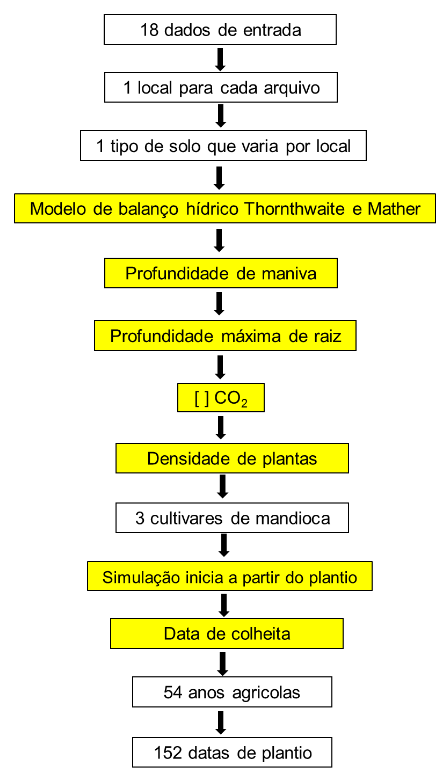
\includegraphics[width=0.4\textwidth]{imagens/SimanihotFlux}
		\caption{Fluxograma do caso de uso 1.}
		\label{fig:SimanihotFlux}}
	\end{figure}

	\bigskip \hrule \bigskip
	%caso 2

	{\bf Caso de Uso 2:} Automação de simulações no modelo SoySim para simular o crescimento, desenvolvimento e produtividade de Soja para o estado do Rio Grande do sul
	\bigskip

	{\bf breve descrição:} Fazer simulações para 37 pontos espalhados no Rio Grande do Sul (37 arquivo de dados meteorológicos), com 120 anos de dados em cada arquivo, de 1980 a 2099, utilizando 7 datas de semeadura (01/08, 01/09, 01/10, 01/11, 01/12, 01/01 e 01/02) e 3 grupos de maturação (4.8, 5.5 e 6.0), em 2 cenários climáticos futuros. Dois conjuntos de dados com 37 arquivos de dados meteorológicos cada um. Dividindo cada um desses 37 arquivos em 3 arquivos com 45 anos de dados, pois o modelo SoySim não suporta fazer a simulação com um arquivo de dados tão extenso.
	\bigskip

	{\bf Fluxo Principal:}

	\begin{enumerate}
		\item Inserir um arquivo de entrada para cada ponto (27\underline51 - 1960\underline2007, 27\underline51 - 2006\underline2053, 27\underline51 - 2052\underline2099, 27\underline52 - 1960\underline2007, 27\underline52 - 2006\underline2053, 27\underline52 - 2052\underline2099 e assim por diante).
		\item Realizar as simulações para os grupos de maturação (4.8, 5.5 e 6.0).
		\item Para cada arquivo de entrada realizar simulações que variam de 01 de agosto até 01 de fevereiro, iniciando na semeadura, de um em um mês
		\item Modificar a densidade de população de plantas para 315.
		\item Depois de preencher estes campos, clicar no botão \emph{run}.
		\item Copiar os dados a partir da linha 14 a 59 do arquivo de resultado “TmpOut.txt” e arazenar todos em um só resultado filtrando itens específicos e gerar um arquivo de resultado com o mesmo.
	\end{enumerate}

	{\bf Fluxo Secundário:}

	\begin{enumerate}
		\item Reiniciar a automação alterando a automação para que a mesma não seja rodada na função de \emph{multiple years} mas sim seja rodada na função de \emph{single years}, onde cada ano precisa ser definido na interface.
		\item Copiar a linha 35 do arquivo resultante “TmpOut.txt” e adicioná-la ao final de um arquivo de resultado único.
	\end{enumerate}

	{\bf Fluxo de exceção:}

	\begin{enumerate}
		\item No caso de encontrar algum alerta de campo preenchido incorretamente, encerrar a automação e envia o usuário para a pós condição.
		\item Caso o modelo apresente um alerta rodando no fluxo principal o programa deve passar para o fluxo secundário
		\item Caso o alerta seja recebido enquanto o modelo já esta no fluxo secundário, passar para o ano seguinte da lista de anos da automação.
		\item Em caso de qualquer interação do usuário durante a tarefa de automação, pausar a simulação e esperar que o usuário recomece a automação ou cancele.
	\end{enumerate}

	\bigskip \hrule \bigskip

	\begin{figure}[!htb]
		{\centering
		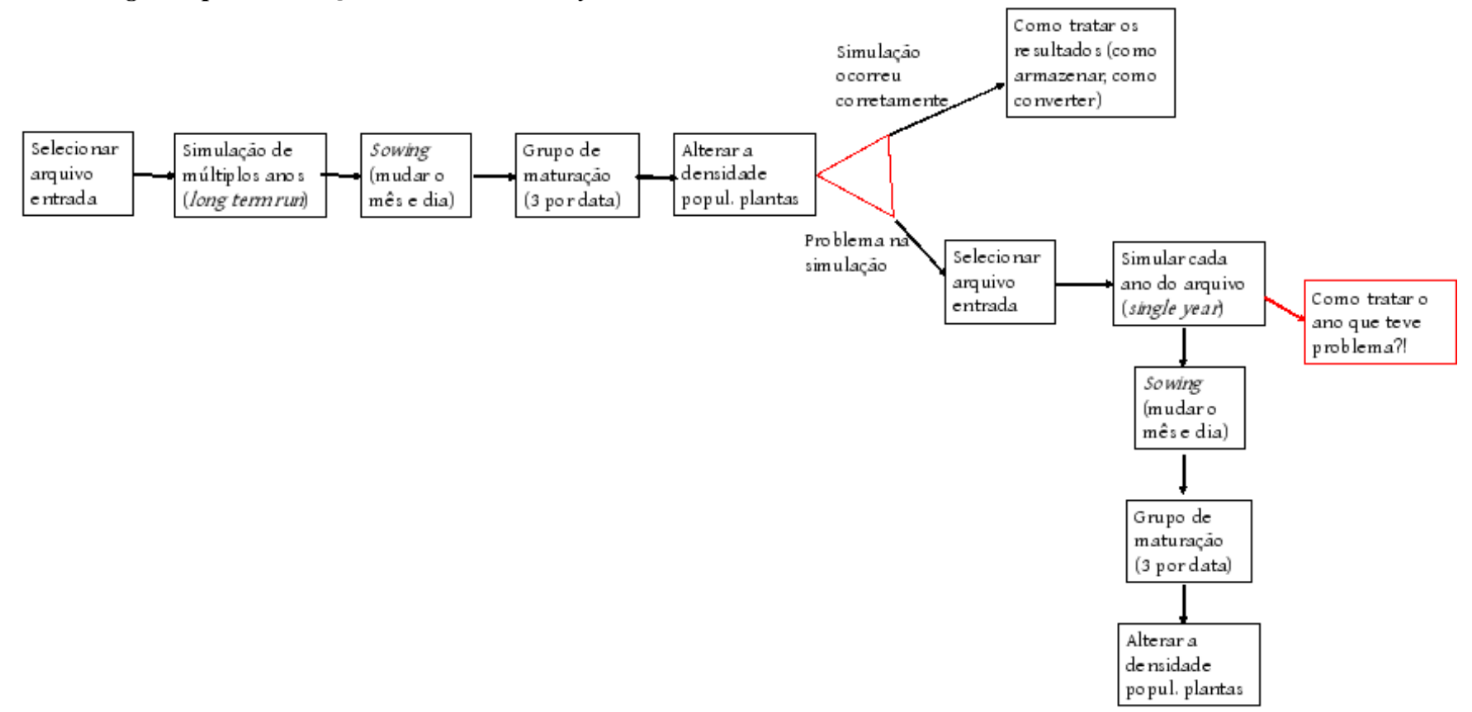
\includegraphics[width=1.0\textwidth]{imagens/SoysimFlux}
		\caption{Fluxograma do caso de uso 2.}
		\label{fig:SoysimFlux}}
	\end{figure}

	\bigskip \hrule \bigskip

	%caso 3

	{\bf Caso de Uso 3:} Automação de simulações no modelo DSSAT para gerar previsões de safra de soja para auxiliar no planejamento agrícola do Estado do Rio grande do Sul
	\bigskip

	{\bf breve descrição:} O RS é um dos Estados brasileiros que mais sente os efeitos dos fenômenos El Nino e La Nina, e atualmente é o terceiro maior responsável pela produção de soja do País. É necessário gerar previsões de safra de soja para auxiliar no planejamento agrícola do Estado do Rio grande do Sul (RS). gerando varias simulações no modelo para diversas datas de semeadura.
	\bigskip

	{\bf Fluxo Principal:}

	\begin{enumerate}
		\item  Abrir o DSSAT, esperar carregar e clicar em \emph{Crop Management Data}. A partir dessa ação, o programa XBuild irá inicializar, e o usuário deve então clicar em New (para começar a criar um novo experimento).
		\item  Criar um nome inexistente para o experimento. \emph{Institute Code} (SM para UFSM), \emph{Site Code} (RS se for dentro do RS), \emph{Year} (2013), \emph{Experiment Number} (99 datas de semeadura), por exemplo. Lembrando que o usuário é livre para escolher a forma de preencher as lacunas dessa etapa do experimento, de uma forma que o torne auto-explicativo. No campo \emph{Crop} (selecione \emph{Soybean}). As demais lacunas podem ser preenchidas com -99.
		\item Nessa etapa o usuário clica em \emph{Environment} e depois em \emph{Fields}. Aqui basicamente deve ser informado qual a série meteorológica o experimento vai utilizar, se existe algum tipo de drenagem e as características do solo daquela região. Ao rodar o modelo para outro local, o usuário deve adicionar mais um “\emph{level}” e repetir o preenchimento com a série meteorológica e as características do segundo local, e assim sucessivamente.
		\item O usuário clica em \emph{Management} e seleciona \emph{Cultivars}, a tela sera redirecionada para uma seção onde deve ser selecionada a cultivar ou as cultivares que serão utilizadas nas rodadas do modelo. Lembrando que essas já devem estar devidamente calibradas pois caso contrário, o nome da cultivar não aparecera na lista de seleção.
		\item Inserção da data ou datas de semeadura, data de emergência, o método utilizado, a forma de distribuição das sementes, a densidade de sementes na semeadura, a densidade de plantas na emergência, o espaçamento entre linhas adotado, a direção das linhas em relação ao Norte e a profundidade de semeadura utilizada para um ou vários experimentos. Lembrando que se o experimento possui alguma característica diferente, esse deve ser inserido como um Novo \emph{Level}.
		\item Determinar a data que o modelo vai começar a simulação do balanço hídrico ou de nutrientes no solo. É aconselhado começar o balanço hídrico no solo entre 20 e 30 dias antes da data de semeadura, buscando uma simulação mais precisa das condições do solo na hora da semeadura.
		\item Selecionar os balanços que gostaria que o modelo realizasse em cada experimento. Aqui pode ser ativado ou não o balanço hídrico, de nitrogênio entre outras. Esses detalhes podem aumentar o desempenho das simulações.
		\item Decidir os métodos que serão utilizados nos balanços que foram selecionados no passo anterior. Se o balanço hídrico foi selecionado, aqui o usuário deve selecionar o método que o modelo deve utilizar para as rodadas em cada experimento. Essa regra também vale para os outros balanços que o usuário deseja que o modelo realize.
		\item Caso o usuário tenha dados mais específicos ou tenha utilizado irrigação em algum dos experimentos que deseja simular, essa é a etapa em que vai inserir as características do manejo utilizado.
		\item Seleciona as informações que serão exibidas no final das rodadas como: Crescimento de massa seca diária, balanço hídrico....entre outros.
		\item Caracterizar cada experimento, identificando cada experimento que vai utilizar a primeira estação meteorológica por exemplo, ou o solo número 1 entre outras informações.
		\item Após realizar essas etapas o usuário deve clicar no botão \emph{Refresh}, que irá atualizar as novas informações e posteriormente pode abrir o programa DSSAT e começar a rodar os experimentos cadastrados.
	\end{enumerate}

	{\bf Fluxo Secundário:}

	\begin{enumerate}
		\item Nenhum
	\end{enumerate}

	{\bf Fluxo de exceção:}

	\begin{enumerate}
		\item No caso de encontrar algum alerta conhecido do modelo tais como alerta de temperatura máxima menor que a mínima, encerrar a automação e envia o usuário para a pós condição.
		\item Em caso de qualquer interação do usuário durante a tarefa de automação, pausar a simulação e esperar que o usuário recomece a automação ou cancele.
	\end{enumerate}

	\bigskip \hrule \bigskip

	\subsection {Aplicação dos casos de uso com outras ferramentas de automação}

	Após a coleta, os casos de uso foram testados em outras ferramentas de automação de tarefas em interfaces gráficas, objetivando compreender em que nível, outras ferramentas indicadas para solucionar o problema exposto nesse projeto, conseguem solucionar os problemas expostos nos casos de uso.

	Como forma de avaliação da inteligibilidade destas ferramentas e o quanto elas se mostram acessíveis aos domínios de conhecimento do usuário, foi proposto aos atores dos casos de uso, que estes tentassem utilizar 3 das ferramentas de automação descritas na revisão literária, descrevendo a experiência de forma objetiva em prós e contras, analisando se foi obtido sucesso ou não e onde os problemas responsáveis pelas falhas se originaram, caso encontrado algum.
	\bigskip


		{\centering \begin{tabular}{ | m{15.6cm} | }
		\hline \\

		{\bf UiPath:} \\ \\
		{\bf Prós:} O programa permite virtualmente a realização de qualquer tarefa, algumas delas intuitivamente sem recorrer a manuais ou tutoriais, tais como construir o fluxo completo de interação com a interface dos modelos fornecendo inclusive lógica suficiente para as repetições e interações necessárias. Nos casos em que foram necessários mover ou reorganizar arquivos para que as rodadas continuassem, também não houve problemas e foi possível organizar intuitivamente. \\ \\
		{\bf Contras:} Definir reações em caso de uma exceção no modelo é uma tarefa complexa e confusa no início, o programa apresenta diversos elementos minimamente diferentes para a realização de tarefas similares, tendo elementos muito carregados e complexos. Sendo intensamente abstrato na programação e contendo poucas funções genéricas comuns a uma linguagem de programação, o UiPath depende completamente do invocamento de métodos externos ao programa para tarefas complexas, podendo recorrer inclusive ao \emph{powershell}. A tarefa de organização dos dados de saida no caso de teste 2 foi simplificada para um manejamento de arquivos. \\ \\

		\hline \hline \\

		{\bf Sikuli:} \\ \\
		{\bf Prós:} O programa é extremamente simples e fácil de entender, é capaz de realizar as tarefas básicas tais como interagir com a interface do modelo e esperar por eventos. \\ \\
		{\bf Contras:} Foi ineficaz em todos os casos de uso por não possuir funcionalidades de lógica básica que permitissem a criação de repetição de eventos de forma sucinta, movimentação e criação de arquivos ou ainda processamento mais complexo de texto necessário a extração dos dados dos arquivos de resultado. \\ \\

		\hline \end{tabular}} \\
	{\centering \begin{tabular}{ | m{15.6cm} | }
		 \hline \\

		{\bf AutoIt} \\ \\
		{\bf Prós:} Novamente um programa capaz de realizar virtualmente qualquer tarefa. \\ \\
		{\bf Contras:}  O programa é totalmente dependente de linguagem \emph{script} tipo BASIC própria, para tarefas mais complexas como as descritas nos casos de uso (\emph{loops},leitura de arquivos, quebra de texto), a automação se torna um desafio possivelmente tão grande quanto o problema original, já que o usuário precisa conhecer com certa profundidade o funcionamento do AutoIt, linguagens de programação, e em especifico a sintaxe e conjunto léxico peculiar usados pela linguagem do programa. \\ \\

		\hline
	\end{tabular}}

	\bigskip
	Analise do caso de uso 2 realizada pelo autor de forma direta nos 3 programas de automação sugeridos sem intervenção de terceiros ou qualquer pessoa do domínio da área:
	\bigskip

	{\centering \begin{tabular}{ | m{15.6cm} | }
		\hline \\

		{\centering {\bf Caso de uso 2 Analisado pelo ator} \\}

		\begin{center} Automação de simulações no modelo SoySim para simular o crescimento, desenvolvimento e produtividade de Soja para o estado do Rio Grande do sul. \end{center}

		\\ \hline \hline \\

		{\bf UiPath:} \\ \\
		{\bf Prós:} Conseguiu fazer com que o software rodasse o SoySim para SingleYear e LongTermRun. Uma rodada sozinha. \\ \\
		{\bf Contras:} Não conseguiu inserir um \emph{loop} para que múltiplas rodadas fossem feitas e apontando que também não conseguiu fazer com que o programa mudassem os arquivos de entrada automaticamente. Além disso, não conseguiu fazer com que o programa entendesse a janela de erro do SoySim. \\ \\

		\hline \end{tabular}} \\ {\centering \begin{tabular}{ | m{15.6cm} | } \hline \\

		{\bf Sikuli:} \\ \\
		{\bf Prós:} consegui montar o scrit que é no mesmo formato do UiPath (visual).  \\ \\
		{\bf Contras:} Na hora de rodar, o programa apresentou um erro que o ator não consegue interpretar, erro apresentado na figura \ref{fig:erroSikuli}. Desistiu da ferramenta devido ao erro. \\ \\

		\hline \hline \\

		{\bf AutoIt} \\ \\
		O ator não conseguiu compreender como a ferramenta funciona, foi capaz de perceber que o programa usa código textual para automatizar as tarefas mas por não ter profundo contato com linguagens de programação ou BASIC, não foi capaz de encontrar uma solução intuitivamente ou em tempo hábil no manual do programa. Desistiu da ferramenta devido a dificuldade. \\ \\

		\hline
	\end{tabular}}

	\begin{figure}[!htb]
		{\centering
		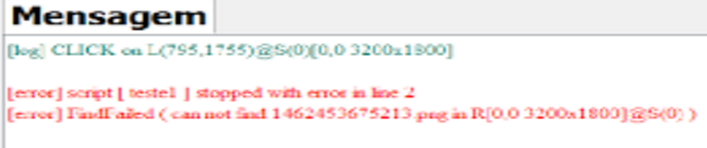
\includegraphics[width=1.0\textwidth]{imagens/sikuli_error}
		\caption{Erro obtido pelo autor no programa Sikuli.}
		\label{fig:erroSikuli}}
	\end{figure}

% ultimas mudancas

    \subsection {Requisitos funcionais elencados}

    Com base nas informações obtidas dos casos de teste e discução com os atores envolvidos foram elencados diversas funcionalidades e por fim foram elencados alguns requisitos funcionais mínimos para a solução dos problemas descritos nos casos de testes dos autores.

    \begin{enumerate}

		\item Deve ser possível salvar ou carregar estruturas de blocos construidos pelo ator de forma que se possa reutilizar automações construidas anteriormente no programa.

		\item Dois blocos, um capaz de executar a ação de clicar uma vez em uma área da tela e outro capaz de executar a ação de clicar duas vezes em uma área da tela, o ator deve ser capaz de escolher a área da tela para cada bloco e o bloco deve usar a área para indicar onde esta clicando.

		\item Um bloco capaz de esperar por uma alteração na tela que indique que o programa pode prosseguir para as próxima tarefas definidas pelo autor.

		%\item Um bloco capaz de mover um arquivo de uma pasta para outra a fim de evitar %que o modelo sobreescreva os resultados durante as simulações.

	\end{enumerate}

    \subsection {Desenvolvimento do software}

    O desenvolvimento do software foi dividido em 3 problemas que definem as principais necessidades do software para que seja possível obter as funcionalidades previstas durante a discução dos requisitos funcionais.

    O primeiro problema a ser solucionado foi a utilização da biblioteca Blockly em uma aplicação local com o objetivo de ter maior acesso aos recursos do sistema.

    Em seguida foi solucionado como realizar a interação com o sistema operacional e as entradas de baixo nível tais como mouse e tecladdo, assim como um método para analizar e pesquisar em imagens para encontrar os locais selecionados pelo usuário onde clicar.

    \subsubsection {Delimitação do escopo}

    Como escopo foram delimitados alguns pré-requisitos necessários para utilizar a solução proposta neste trabalho, onde, o sistema deve ser uma aplicação desenvolvida usando Java e Javascript.

    \subsubsection {Blockly em uma aplicação Java}

    Em um primeiro momento, com o objetivo de rodar o Blockly, uma biblioteca Javascript 100\% \emph{client side} dependente de um ambiente web, em uma aplicação java, optou-se por uma solução que envolve uma aplicação JavaFX com um cliente Web embutido, descrita de forma geral na imagem \ref{fig:struct}.

    \begin{figure}[!htb]
        {\centering
        \includegraphics[width=1.0\textwidth]{imagens/struct.png}
        \caption{Estrutura geral da solução.}
        \label{fig:struct}}
    \end{figure}

    O software ao iniciar carrega a a pagina da aplicação web desenvolvida com base na biblioteca Blockly em uma instância da classe \texttt{WebEngine}, contida na plataforma JavaFX, sendo que esta instância pertencente a um objeto da classe \texttt{WebView} também contida na plataforma JavaFX, responsável pela gestão e renderização da página na interface gráfica de uma aplicação JavaFX.

    Foi utilizada a funcionalidade LiveConnect, presente na maioria dos navegador web, que permite a comunicação entre o navegador e aplicativos java para conectar o software e a aplicação web. Foi desenvolvida a classe \texttt{JavascriptMsgr} com o objetivo de estabelecer os métos de comunicação entre a aplicação web e o software, contendo uma referência para o objeto instanciado da classe \texttt{javafx.scene.web.WebEngine} com o qual cria um objeto \texttt{netscape.javascript.JSObject} que tornar a classe \texttt{JavascriptMsgr} visível para a aplicação web.

    A classe \texttt{JavascriptMsgr} trata tanto as mensagens vindas da aplicação web como as mensagens enviadas do software, a imagem \ref{code:javascriptmsg.java} apresenta dois exemplos de métodos presentes na classe \texttt{JavascriptMsgr} em trechos distintos\footnote{código completo disponível em https://github.com/RomuloPBenedetti/TCC/tree/master/Software/src/main/java/automata}, onde o primeiro envia uma mensagem para a aplicação web e o segundo recebe uma mensagem.


\begin{figure}[!htb]
\begin{lstlisting}
    // método que envia uma String contendo o arquivo xml gerado na ultima vez em que foi
    // salvo a blockly.mainWorkspace

    public void loadBlocks(String xml) {
        com.sun.javafx.application.PlatformImpl.runAndWait(() ->{
            String escaped = StringEscapeUtils.escapeEcmaScript(xml);
            engine.executeScript("loadBlocks(\""+ escaped +"\")");
        });
    }

    // método que recebe um pedido para esperar enquanto não localizar uma imagem na
    // pasta raiz, recebe um endereço relativo na pasta raiz do software e um valor
    // de intervalo em milisegundos que deve esperar a cada procura sem sucesso
    public void waitImg (String imgSrc, int milisec){
        try {
            BufferedImage target = null;
            target = ImageIO.read(new File(imgSrc.substring(3)));
            BufferedImage screenshot =
                robot.createScreenCapture(primaryScreenBounds);
            ImageSearch is = new ImageSearch(target);

            while(is.search(screenshot)[0] == -1){
                screenshot = robot.createScreenCapture(primaryScreenBounds);
                System.out.println("tried");
                Thread.sleep(milisec);
            }
            System.out.println("match!");
        } catch (IOException | InterruptedException e) {
            e.printStackTrace();
        }
    }
\end{lstlisting}
    \caption{2 métodos da classe mediadora da comunicação entre a aplicação web e o software}
	\label{code:javascriptmsg.java}
\end{figure}

    A classe possui diversos métodos que extentem as funcionalidades da aplicação web e permitem ao foftware utilizar a biblioteca blockly para fornecer a biblioteca visual, gerar e executar código.

    \subsubsection {Interação e pesquisa por regiões na tela do sistema operacional}

    A interação com o Sistema operacional é realizada por instâncias da classe import \texttt{java.awt.Robot} capaz de gerar eventos de sistema nativos. Apesar de ter sido desenvolvida com o objetivo principal de realizar testes automatizados e aplicações auto-executáveis, por ser capaz de manipular mouse e teclado a nível de sistema, pode ser utilizada para qualquer tarefa que busque automatizar o controle do sistema operacional.

    Para encontrar as áreas a serem clicadas ou regiões a serem observadas na espera de uma mudança, foi desenvolvida a classe \texttt{ImageSearch} com uma solução própria de pesquisa otimizada para imagens, que analiza uma imagem capturada da tela do sistema em busca de referências exatas das áres escolhidas pelos usuários.

    Diversas outras soluções foram analizadas como a biblioteca OpenCV\cite{openCV} ou ainda o framework brasileiro de processamento de imagens em Java, Marvin\cite{marvin}. Porêm outras soluções traziam diversos problemas que não se justificavam, variando da necessidade de mais bibliotecas, adaptação a uma abordagem mais complicada e distante da necessidade do projeto ou ainda limitações em termos de plataformas

    A abordagem é descrita na figura \ref{fig:ImageSearch} se trata de extrair da área selecionada pelo usuário, dois pixels, um com o maior valor de cor RGB dentre todos e outro com o menor valor dentre todos, assim como a distância 'x' e 'y' destes dois pixels da origem. Por questões de otimização as cores nas imagens são analizadas como se fossem inteiros absolutos de 32 bits.

    Posteriormente percorre todos os pixels da imagem que dão acesso a uma região do tamanho da áre capturada (de x = 0 até x = (larguraCaptura - larguraArea)), usando a posição em que se encontra como âncora para verificar nas posições salvas se os 2 pixels extraidos da área são iguais aos pixels na posição da imagem.

    Caso os 2 pixels sejam iguais, inicia-se uma análixe de uma malha esparça de pixels na área, onde é somado a diferença dos pixels da imagem extraida pelo usuário e a imagem capturada da tela, caso a diferença no final for zero, significa que foi encontrado uma área na imagem capturada, igual a imagem da áre que o usuário escolheu e neste caso a função retorna a posição 'x' 'y' da âncora.

    Os métodos principais da classe \texttt{ImageSearch}\footnote{código completo disponível em https://github.com/RomuloPBenedetti/TCC/tree/master/Software/src/main/java/automata}, podem ser observados na imagem \ref{code:ImageSearch.java}.

    \begin{figure}[!htb]
        {\centering
        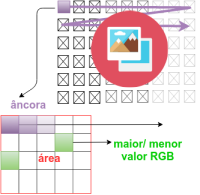
\includegraphics[width=0.3\textwidth]{imagens/searchImage.png}
        \caption{descrição visual da tarefa realizada pela classe \texttt{ImageSearch}.}
        \label{fig:ImageSearch}}
    \end{figure}

    \begin{figure}[!htb]
    \begin{lstlisting}

        public final void storeTarget(BufferedImage t) {
        this.t = t; int rgb; tWidth = t.getWidth(); tHeight = t.getHeight();
        for(int x = 0; x < tWidth; x++) {
            for (int y = 0; y < tHeight; y++) {
                rgb = t.getRGB(x, y);
                if (Integer.compareUnsigned(rgb, max)>0) { max = rgb; maxX = x; maxY = y; }
                if (Integer.compareUnsigned(rgb, max)<0) { min = rgb; minX = x; minY = y; }
            }
        }
    }

    public final int[] search(BufferedImage i) {

        int iWidth, iHeight, point[] = new int[2];
        point[0] = -1; point[1] = -1;
        int startX[] = new int[cores], endX[] = new int[cores];
        int startY[] = new int[cores], endY[] = new int[cores];

        iWidth = i.getWidth()-tWidth; iHeight = i.getHeight()-tHeight;
        ExecutorService executor = Executors.newFixedThreadPool(cores);

        for (int q = 0 ; q < cores ; q++){
            startX[q] = (iWidth/cores)*q; startY[q] = 0;
            endX[q] = (iWidth/cores)*(q+1); endY[q] = iHeight;
            int fQuad = q;

            executor.execute(() -> {
                Thread.currentThread().setName("thread" + fQuad);
                int difference = 100; int rgbC;
                for (int x = startX[fQuad]; x < endX[fQuad]; x++) {
                    for (int y = startY[fQuad]; y < endY[fQuad]; y++) {
                        rgbC = i.getRGB(x + maxX, y + maxY);
                        if (rgbC == max) {
                            rgbC = i.getRGB(x + minX, y + minY);
                            if (rgbC == min) {
                                difference = 0;
                                for (int ty = 0; ty < tHeight; ty = ty +3) {
                                    for (int tx = 0; tx < tWidth; tx = tx +3) {
                                        difference += t.getRGB(tx, ty) - i.getRGB(x+tx, y+ty);
                                    }
                                }
                                if (difference == 0) {
                                    point[0] = x; point[1] = y;
                                    executor.shutdownNow();
                                }
                            }
                        }
                        if (difference == 0) break;
                    }
                    if (difference == 0) break;
                }
            });
        }
        try {
            executor.awaitTermination(1, TimeUnit.SECONDS);
        } catch (InterruptedException e) {
            e.printStackTrace();
        }
        return point;
    }
    \end{lstlisting}
        \caption{Métodos que analisam a imagem da área e a imagem capturada da tela do sistema}
    	\label{code:ImageSearch.java}
    \end{figure}

    O método \texttt{StoreTarget} percorre a imagem que o usuário selecionou para ser clicada ou analizada e compara o valor de cada pixel com variáveis auxiliares, onde posteriormente sobrescreve o valor destas váriaveis se o pixel for realmente um valor maior ou menor do que os considerados anteriormente.

    Já o método \texttt{search} procura pelo máximo ou mínimo na imagem capturada pelo software, quando encontra a área que contem nas mesmas posições o valor máximo e mínimo, analisa a área um pixel a cada 3, caso a soma de todas as diferenças da área de um valor 0 todas as \emph{threads} são paradas e a posição do pixel âncora ou origem da área é retornado. A tarefa também é dividia entre os núcleos do processador do usuário para obter melhor performance e o metodo apenas retorna quando o todas as \emph{threads} iniciadas pela pesquisa terminarem.

    \subsubsection {modelagem das funcionalidades no softwares}

    A interface do software foi desenvolvida para ser o mais simples e limpa possível com o objetivo de diminuir duvidas ou confusão dos usuários, existem, alem do botão nativo de lixeira, 3 botões a mais, um para executar a simulação, um para carregar um quebra-cabeças que tenha sido salvo em e outro para salvar um quebra-cabeças atual. O programa utiliza o único formato de armazenamento em arquivo disponivel na biblioteca blockly, a linguágem de marcação XML. É possível ver a interface na figura \ref{fig:app}.

    \begin{figure}[!htb]
        {\centering
        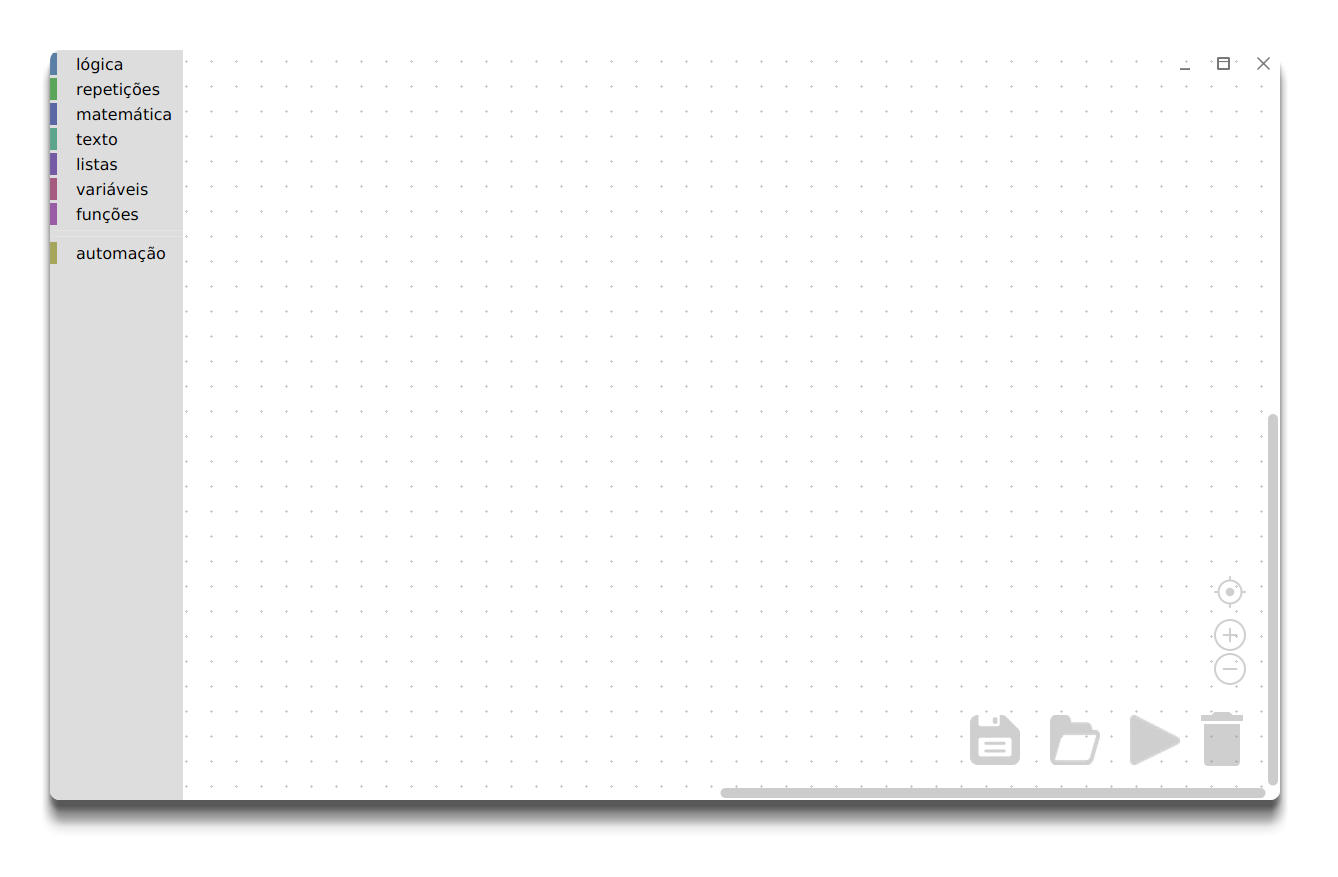
\includegraphics[width=1.0\textwidth]{imagens/app.png}
        \caption{Blocos construidos para as operações de automação}
        \label{fig:app}}
    \end{figure}

    para fornecer as funcionalidades foram definidos quatro blocos que expressam funcionalidades fundamentais para a automatização, dois blocos que expressam a abilidade de clicar em algum lugar da interface, um para clique duplo e outro para clique único, também, um bloco que permite esperar por algum evento visual, para que seja possível esperar a finalização do processamento dos modelos, e por ultimo um bloco que permite digitar texto na entrada de texto do sistema operacional.

    É possível observar os blocos na imagem \ref{fig:myblocks} e a descrição formal em javascript destes blocos nas figura \ref{code:myBlocks.js}\ref{code:myBlocksGenerator.js}\footnote{código completo disponível em https://github.com/RomuloPBenedetti/TCC/tree/master/Software/src/main/resources/blocklyResource}.

    \begin{figure}[!htb]
        {\centering
        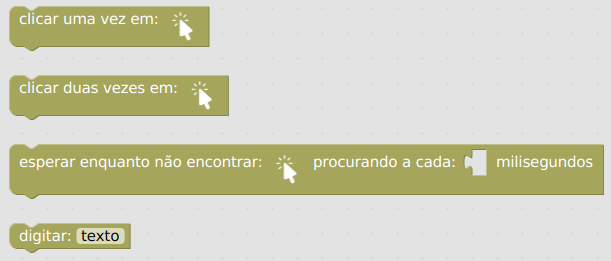
\includegraphics[width=1.0\textwidth]{imagens/blocks.png}
        \caption{Blocos construidos para as operações de automação}
        \label{fig:myblocks}}
    \end{figure}

    \begin{figure}[!htb]
    \begin{lstlisting}
        Blockly.Blocks['click_single_special'] = {
          init: function() {
            this.appendDummyInput("imageInput")
                .appendField("clicar uma vez em:")
                .appendField(new Blockly.FieldImageButton("../images/icons/clickBlack.png", 30, 30, "", imageButtonEvent), "FieldImageButton");
            this.setPreviousStatement(true, null);
            this.setNextStatement(true, null);
            this.setColour(60);
            this.setTooltip('Procura na sua tela pela região que a imagem representa e clica no centro uma veze, para escolher, clique na imagem branca do bloco, va ao local desejado aperte ctrl+shift+c, selecione onnde clicar com o mouse e aperte enter.');
          }
        };

        Blockly.Blocks['click_doble_special'] = {
          init: function() {
            this.appendDummyInput("imageInput")
                .appendField("clicar duas vezes em:")
                .appendField(new Blockly.FieldImageButton("../images/icons/clickBlack.png", 30, 30, "", imageButtonEvent), "FieldImageButton");
            this.setPreviousStatement(true, null);
            this.setNextStatement(true, null);
            this.setColour(60);
            this.setTooltip('Procura na sua tela pela região que a imagem representa e clica no centro duas vezes, para escolher, clique na imagem branca do bloco, va ao local desejado aperte ctrl+shift+c, selecione onnde clicar com o mouse e aperte enter.');
            console.log(this.id);
          }
        };

        Blockly.Blocks['text_typer'] = {
          init: function() {
            this.appendDummyInput("textToType")
                .appendField("digitar:")
                .appendField(new Blockly.FieldTextInput("texto"), "text");
            this.setPreviousStatement(true, null);
            this.setNextStatement(true, null);
            this.setColour(60);
            this.setTooltip('');
            this.setHelpUrl('http://www.example.com/');
          }
        };

        Blockly.Blocks['Image_Wait'] = {
          init: function() {
            this.appendDummyInput("imageInput")
                .appendField("esperar enquanto não encontrar:")
                .appendField(new Blockly.FieldImageButton("../images/icons/clickBlack.png", 30, 30, "", imageButtonEvent), "FieldImageButton");
            this.appendValueInput("miliToWait")
                .setCheck("Number")
                .setAlign(Blockly.ALIGN_RIGHT)
                .appendField("procurando a cada:");
            this.appendDummyInput()
                .appendField("milisegundos");
            this.setInputsInline(true);
            this.setPreviousStatement(true, null);
            this.setNextStatement(true, null);
            this.setColour(60);
            this.setTooltip('para escolher por que imagem esperar, clique na imagem branca do bloco, va ao local desejado aperte ctrl+shift+c, selecione onnde clicar com o mouse e aperte enter.');
            this.setHelpUrl('http://www.example.com/');
          }
        };
    \end{lstlisting}
        \caption{Descrição dos blocos na aplicação web e seus respectivos geradores de código}
        \label{code:myBlocks.js}
    \end{figure}

    \begin{figure}[!htb]
    \begin{lstlisting}
        Blockly.JavaScript['click_doble_special'] = function(block) {
          src = (block.getFieldValue('FieldImageButton')).replaceAll("\\\\","\\\\");
          running = 'if (running) {\n';
          calling = '    running = java.clickIn(\"' + src + '\",' + 2 + ');\n';
          end =     '}\n';
          var code = running + calling + end;
          return code;
        };

        Blockly.JavaScript['click_single_special'] = function(block) {
          src = (block.getFieldValue('FieldImageButton')).replaceAll("\\\\","\\\\");
          running = 'if (running) {\n';
          calling = "java.clickIn(\"" + src + '\",' + 1 + ');\n';
          end =     '}\n';
          var code = running + calling + end;
          return code;
        };

        Blockly.JavaScript['text_typer'] = function(block) {
          text = block.getFieldValue('text');
          running = 'if (running) {\n';
          calling = "    running = java.type(\"" + text + '\");\n';
          end =     '}\n';
          var code = running + calling + end;
          return code;
        };

        Blockly.JavaScript['Image_Wait'] = function(block) {
          src = (block.getFieldValue('FieldImageButton')).replaceAll("\\\\","\\\\");
          milisec = Blockly.JavaScript.valueToCode(block, 'miliToWait', Blockly.JavaScript.ORDER_ATOMIC) || '0'
          running = 'if (running) {\n';
          calling = '    java.waitImg(\"' + src + '\", '+ milisec + ');\n';
          end =     '}\n';
          var code = running + calling + end;
          return code;
        };
    \end{lstlisting}
        \caption{Geradores de código java dos blocos construidos}
        \label{code:myBlocksGenerator.js}
    \end{figure}

    Como é possível ver o bloco \texttt{Image\_Wait} e os blocos que representam as ações de clique de mouse, \texttt{click\_doble\_special} e \texttt{click\_single\_special} utilizam um campo próprio chamado \texttt{FieldImageButton}, desenvolvido observando-se o campo original presente na biblioteca Blockly \texttt{field\_image}\footnote{o código desta classe pode ser encontrado em https://github.com/google/blockly/}, este campo adiciona a imagem um \emph{eventListenner} que ao ser clicado envia ima mensagem que da início a tarefa de captura de tela no software, que ao ser terminada pelo usuário, envia uma mensagem contendo o caminho da imagem da área selecionada pelo usuário que deve sofrer a ação do bloco junto com suas dimensões. Por sua vez a aplicação web atualiza a imagem do bloco para reresentar a área que o usuário escolheu.

    Toda a tarefa é mantida coêsa transferindo junto com estas mensagens o ID único que a própria biblioteca Blockly gera para cada bloco assim tanto a aplicação web como o software sempre sabem para que bloco é cada mensagem. Por questões de flexibilidade e simplicidade foi decidido utilizar a linguagen Javascript por questões de simplicidade já que é uma das linguagens nativas do software e disponível para os outros blocos da biblioteca por padrão ja.

    Quando o usuário clica no botão para executar o modelo no software, é enviado uma mensagem para a aplicação web, pedindo que para que a biblioteca Blockly monte o código com base no quebra-cabeça montado e por fim, execute o código com a função \texttt{eval}.

    Como é possível observar, os geradores de código voram construidos para realizar chamadas no no software java e portanto, a aplicação web fica responsável apenas pela montagem da lógic que guia a execução das tarefas tais como construção de repetições ou definições de valores a serem enviados junto as mensagens para que o software as realize. É possível ver um exemplo do código gerado por um conjunto de blocos na figura\ref{fig:myblocks}.

    \begin{figure}[!htb]
        {\centering
        \includegraphics[width=1.0\textwidth]{imagens/blocksandcode.png}
        \caption{Blocos construidos para as operações de automação}
        \label{fig:blocksAndCode}}
    \end{figure}

    \chapter {Resultados}

    \subsection {Validando solução com os casos de teste}

    Com as funcionalidades desenvolvidas no software não é possível solucionar todas as questões desenvolvidas nos casos de teste dos 3 modelos Porem é possível solucionar em geral o problema do modelo Simanihot. Que apenas exige interações de digitação e cliques na interface gráfica do sistema.

    \subsection {Simanihot}

    \chapter {Conclusão}

    A proposta inicial deste trabalho consistia principalmente em apresentar uma solução de automação de interfaces gráficas de forma simplificada com base na biblioteca de programação visual Blockly dentro do contexto de modelos de simulação de culturas agrícolas. Entretantoo resultado final desta pesquisa não trata-se não de uma solução completa, mas de um software que oferece a possibilidade de automatização de alguns problemas. Conclusão tomada durante o desenvolvimento, a partir dos percalços e da análise constante da amplitude da proposta e das necessidades durante a validação das abordagens em questão.

    Como contribuição este trabalho apresentou uma abordagem diferenciada na programação de tarefas automatizadas expondo de forma mais simplificada lógica comum em linguagens de programação e \emph{script} tradicionais, fornecendo uma ferramenta que pode descrever de forma muito flexível interações com a interface gráfica e permitindo em algum nível realizar a automatização de parte das tarefas maçantes presentes na interação com interfaces gráficas de modelos matemáticos de simulação de culturas agrícolas mais simples.

    A lista a segir expõe em ordem de relevância algumas melhorias que poderiam ser incorporadas em uma nova versão deste projeto:

    \begin{itemize}
    	\item tratar arquivos com conteudo de texto, permitindo copiar arquivos para outros locais, criar novos arquivos com novas informações, renomeá-los e processar e extrair informações destes textos.
    	\item Fornecer \emph{feedback} visual ao finalizar automatizações ou receber erros durante a execução de uma automatização.
        \item Expandir a interação com o sistema operacional de forma que o software possa procurar dentre diversas janelas, interaja de forma mais consistente em outras plataformas.
    	\item Obter uma forma mais eficiente de captura de tela já que a captura de tela realizada pela classe \texttt{Robot} alem de lenta pode produzir artefatos e não capturar alguns elementos dinâmicos de alguns programas.
        \item Oferecer blocos que simplifiquem elementos lógicos já presentes na biblioteca Blockly permitindo a formulação de quebra-cabeças de automatização mais simples.
        \item Refinar os pequenos detalhes em geral da aplicação com salvamento e carregamento de quebra-cabeças ou fornecimento de configurações para troca de idioma.
    \end{itemize}

	\setlength{\baselineskip}{\baselineskip}
	\bibliographystyle{abnt}
	\bibliography{andamento}
\end{document}
